\documentclass[conference,compsoc]{IEEEtran}
\usepackage[utf8]{inputenc}
\usepackage[T1]{fontenc}
\usepackage{lineno,hyperref}
\usepackage{amssymb}
\usepackage[inline]{enumitem}
\usepackage[linesnumbered,ruled,vlined]{algorithm2e}
\usepackage{epstopdf}
\usepackage{amsmath}
\usepackage{tabularx}
\usepackage{multirow}
\usepackage{float}
\usepackage{graphicx}
\usepackage{filecontents}
\usepackage{cite}
\begin{document}

\title{New strategies for survivable green Fiber-Wireless networks}

\author{\IEEEauthorblockN{Vit\'{o}ria Alencar de Souza}
\IEEEauthorblockA{Department of electrical engineering
Federal University of Par\'{a}\\
Bel\'{e}m - Brazil \\
Email: vitoria.souza@itec.ufpa.br}
}
\maketitle

%%%%%%%%%%%%%%%%%%%%%%%%%%%%%%%%%%%%%%%%%%%%%%%%%%%%%%%%%%%%%%%%%%%
\begin{abstract}
As the communications has improved the human behavior also changed and it is also creating new demands and new challenges for the next generation of broadband access.
Fiber-Wireless (FiWi) broadband networks might be used in the next generation of broadband access in order to provide efficient mobile access and the challenge is provide a FiWi standard whose could be efficient and survivable providing high bit rates  and  also is concerned  about  the environment's needs.
\end{abstract}

\IEEEpeerreviewmaketitle

\section{Introduction}

As concerns about climate change, rising fossil fuel prices and energy security increase, companies 
and governments around the world are committing great efforts to develop new technologies for the 
green strategies addressing climate chance globally and facilitating low greenhouse gas(GHG) 
development. Currently, the GHG emissions produced by the Information and Communication Technology 
(ICT) industry alone are said to be equivalent to the GHG emissions of the entire aviation industry 
~\cite{yu2012green}.


The passive optical network (PON) is a promising technology for broadband access as it can offer 
higher bandwidth to end users than other alternatives such as DSL and cable TV networks. 

The PON is point-to-multipoints and generally there is a single transceiver in the optical line 
terminal (OLT) in the central office (CO). The OLT sends information to the optical network units 
(ONUs) located at the subscriber end.
Traditional PONs are time division multiplexing PONs (TDM-PONs), in which a single wavelength is 
used for all down-stream transmissions and another wavelength is used for all upstream 
transmissions. The upstream bandwidth is shared among the users in the manner of time division 
multiplexing.

Various TDM-PON technologies have been developed, including ATM PON (APON), broadband PON (BPON), 
gigabit PON (GPON), and Ethernet PON (EPON). As end users demand more bandwidth, there is the need 
to further increase the PON bandwidth using wavelength division multiplexing (WDM) \cite{5759821}.

Then in order to provide more efficient communications services as reduce the GHG development, Fiber-Wireless (FiWi) broadband access network could be in the future a promising "last mile" access technology, because it might integrates wireless and optical access technologies in terms of their respective merits, such as high capacity and stable transmission from optical access technology, and easy deployment and flexibility from wireless access technology. 

Since FiWi is expected to carry a large amount of traffic and low energy bit coast, numerous traffic flows may be interrupted by the failure of network components. Thus, survivability  joint with the reduction of the GHG in FiWi is a key issue aiming at reliable, robust  and green service ~\cite{Liu201268}.



\section{Joint Fiber-Wireless broadband access network}
Fiber-wireless (FiWi) is an access networks offer to combine the robustness and 
high capacity of optical access networks with mobility, ubiquity and 
flexibility of the wireless access networks in the last mile of the Internet.

A FiWi network consists of an optical back-end that employs a passive optical network 
(PON) technology, such as Ethernet PON (EPON) or wavelength-division multiplexing (WDM)-PON, and a 
wireless front-end technology, such as
IEEE 802.11g, IEEE 802.16j, IEEE 802.16m, Third Generation
Partnership Project (3GPP) Long Term Evolution (LTE), or LTE-Advanced 
(LTE-A)~\cite{4785396}.

\begin{figure}[H]
 	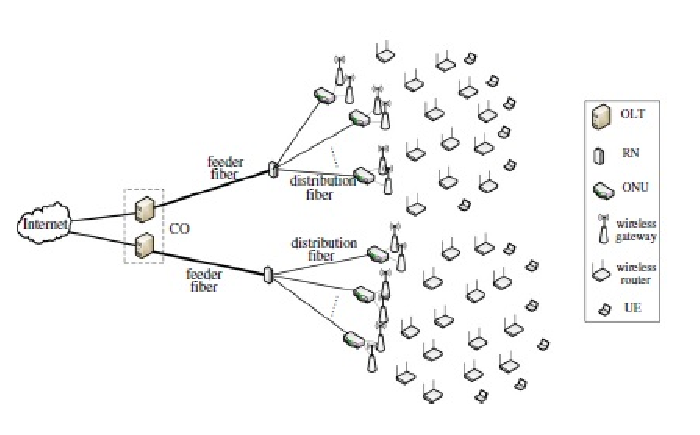
\includegraphics[width=\linewidth]{fiwi.eps}
 	\caption{A typical FiWi architecture ~\cite{Liu201268}.}
 	\label{fig:fiwi_arch}
\end{figure}

\section{Survivable strategies for FiWi networks}% what means and how?
A survivable network can deal with the failures of the active components in a network.
An important design problem arising from the proposed
protection scheme is to determine the pairs of backup ONUs
to be connected with fibers so that :
\begin{itemize}
\item The amount of traffic that can be protected upon an OLT/ONU failure is maximized.
             
\item The cost of connecting the backup ONUs is minimized
\end{itemize}

We refer to this problem as the maximum protection withh
minimum cost (MPMC) problem \cite{5759821}.
Some types of optimization algorithms could be used to reach the minimum
standard FiWi networks.

Othe kind of problem statement could be created for solve the survivable problem such as routing 
algorithms 
and others  in order to minimize the power consume in a FiWi network.



\section{Green strategies for FiWi networks}% what means and how?
Green strategies for FiWi systems concern in enhance energy efficiency, 
evolve the resource management, utilize relay techniques, cross-layer design 
and optimization, rate adaptation, graph-theoretic, router architecture, 
dynamic scheduling or smart grid communications to power save the FiWi 
networks ~\cite{yu2012green}.

Energy efficiency in access networks in FiWi networks has three aspects that could be enhanced in 
order to achieve the maximum efficient FiWi network:


\subsection{Using energy-efficient architectures  leading to a power saving system}
This kind of study proposes different architectures in order to switches the ONUs in the networks.

In the article~\cite{sleepmode} was designed a architecture that uses a analog circuit to switches 
on/off the ONU in order to power-saving 3.1 W. Otherwise this circuit introduces a 5 ms delay.

The article ~\cite{sleepmode} also proposes a second architecture that uses fast recovery, but this 
solution is more expense because it uses a sleep control circuit whose is
employed together with a burst mode clock and data recovery circuit (BM-CDR), which sets a counter 
to control the sleep duration and generates a wakeup signal for the sleep control circuit, this 
solution leads saving of 2.77W and a delay of 0.125 ms.


\subsection{Energy-efficient design and planning}
 
 This kind of study aims learn the standards of the network and programming when put the network in 
 mode on. Then it is an alternative and leads to a higher power saving systems.
 
 In ~\cite{5424000} his study takes advantage of variable traffic profiles on the wireless 
routers and gateways throughout the day, this study aims learn the existing dynamic profile of the 
 traffic and then put maximum of ONUs to sleep in slot of time.
 
 
\subsection{Energy-efficient medium access control (MAC)/routing protocols }

 The study of energy-efficient medium access control (MAC)/ routing protocols proposes green 
routing algorithms.

According to the proposed green algorithm, a packet is
routed toward the heavily loaded routers so that some gateways
can be left lightly loaded, and their ONUs can be put in sleep
mode by the OLT whose determines that traffic load on
an ONU is above a heavy load watermark, it sends a WAKEUP
signal to an ONU in order to avoid long packet delays and losses ~\cite{fiwienergyeficient}.





  
\section{Survivable-Green strategies for FiWi networks}% what means and 

The next generation of broadband networks are expected to  high providing support for a massive 
range of services. Industry transformation, digitalization, the global dependence on mobile 
broadband, mtc, the iot, and the rise of innovative industrial applications all require new 
services, which has a considerable impact on the transport network ~\cite{5greview}.

So the challenge is improve communications capacity and his penetrability and be carefull with the 
environment.

In the figure \ref{fig:fiwi_iot} are showed the future needs of telecommunications demands, the 
traffic has increased and the new communications standards has the challenge off be green in order 
to take care of environment.



\begin{figure}[H]
 	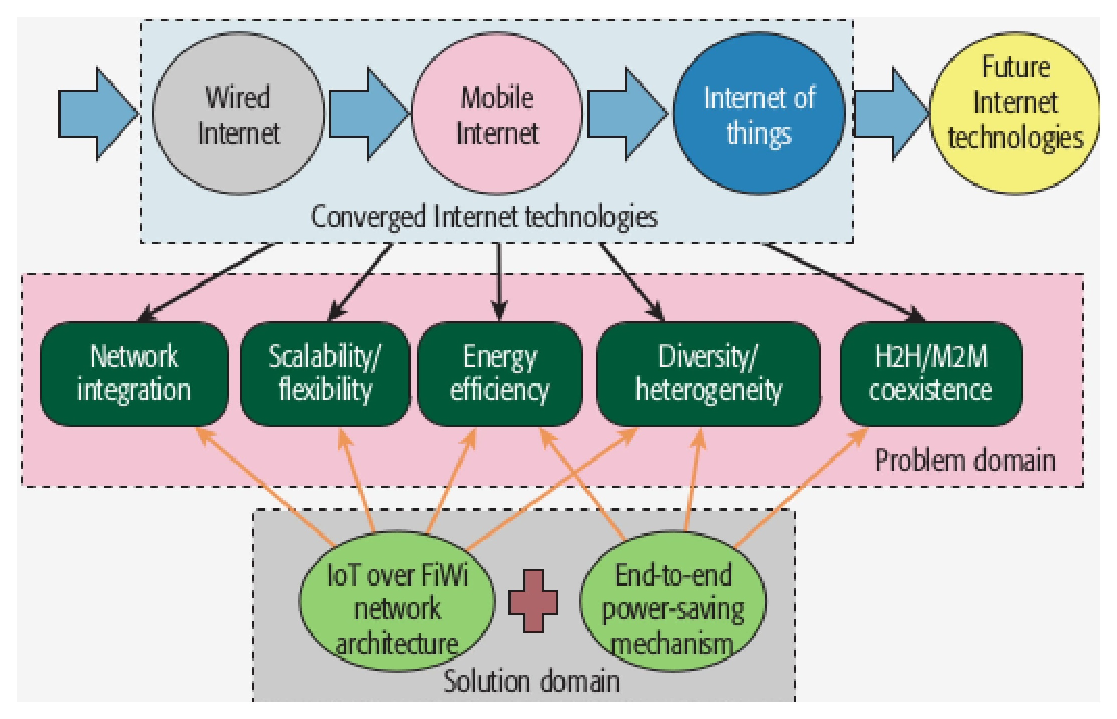
\includegraphics[width=9cm]{future.eps}
 	\caption{Overview of key challenges in the integrated IoT over FiWi 
acess networks ~\cite{iot_fiwi}.}
 	\label{fig:fiwi_iot}
\end{figure}


In this section are showed many posible solutions that could lead to green survivable FiWi networks 
in the future.

\subsection{Auxiliary graph for green survivability in FiWi}

%
\subsection{Green survivability scheme based on backup resource in optical back-end}


\subsubsection{Traffic prediction model}
\subsubsection{Backup ONUs selection}
\subsubsection{Backup fibers deployment}



%
\subsection{Green survivability scheme based on self-healing in wireless front-end}

\subsubsection{Protection against distribution fiber failure}
\subsubsection{Protection against feeder fiber failure}
\subsubsection{Protection against wireless node failure}


%
\subsection{Green survivability scheme based on joint wireless-optical
protection}

\subsubsection{Intra-segment differentiated protection}
\subsubsection{Inter-segment differentiated protection}
\subsubsection{Joint intra- and inter-segment differentiated protection}



\section{Conclusion}
The conclusion goes here.


\bibliographystyle{./IEEEtran}
\bibliography{./IEEEabrv,./telecom.bib,./dsp.bib}
\end{document}

